\documentclass{article}

\usepackage{graphicx}
\usepackage{tikz}
\usepackage{tikzsymbols}
\usetikzlibrary{calc,patterns,shapes.geometric}
\pagestyle{empty}
\usepackage[margin=0pt]{geometry}
\geometry{papersize={14in,12in}}

\def\centerarc[#1](#2)(#3:#4:#5){\draw[#1] ($(#2)+({#5*cos(#3)},{#5*sin(#3)})$) arc (#3:#4:#5);}

\begin{document}
	\begin{figure}
		\centering
		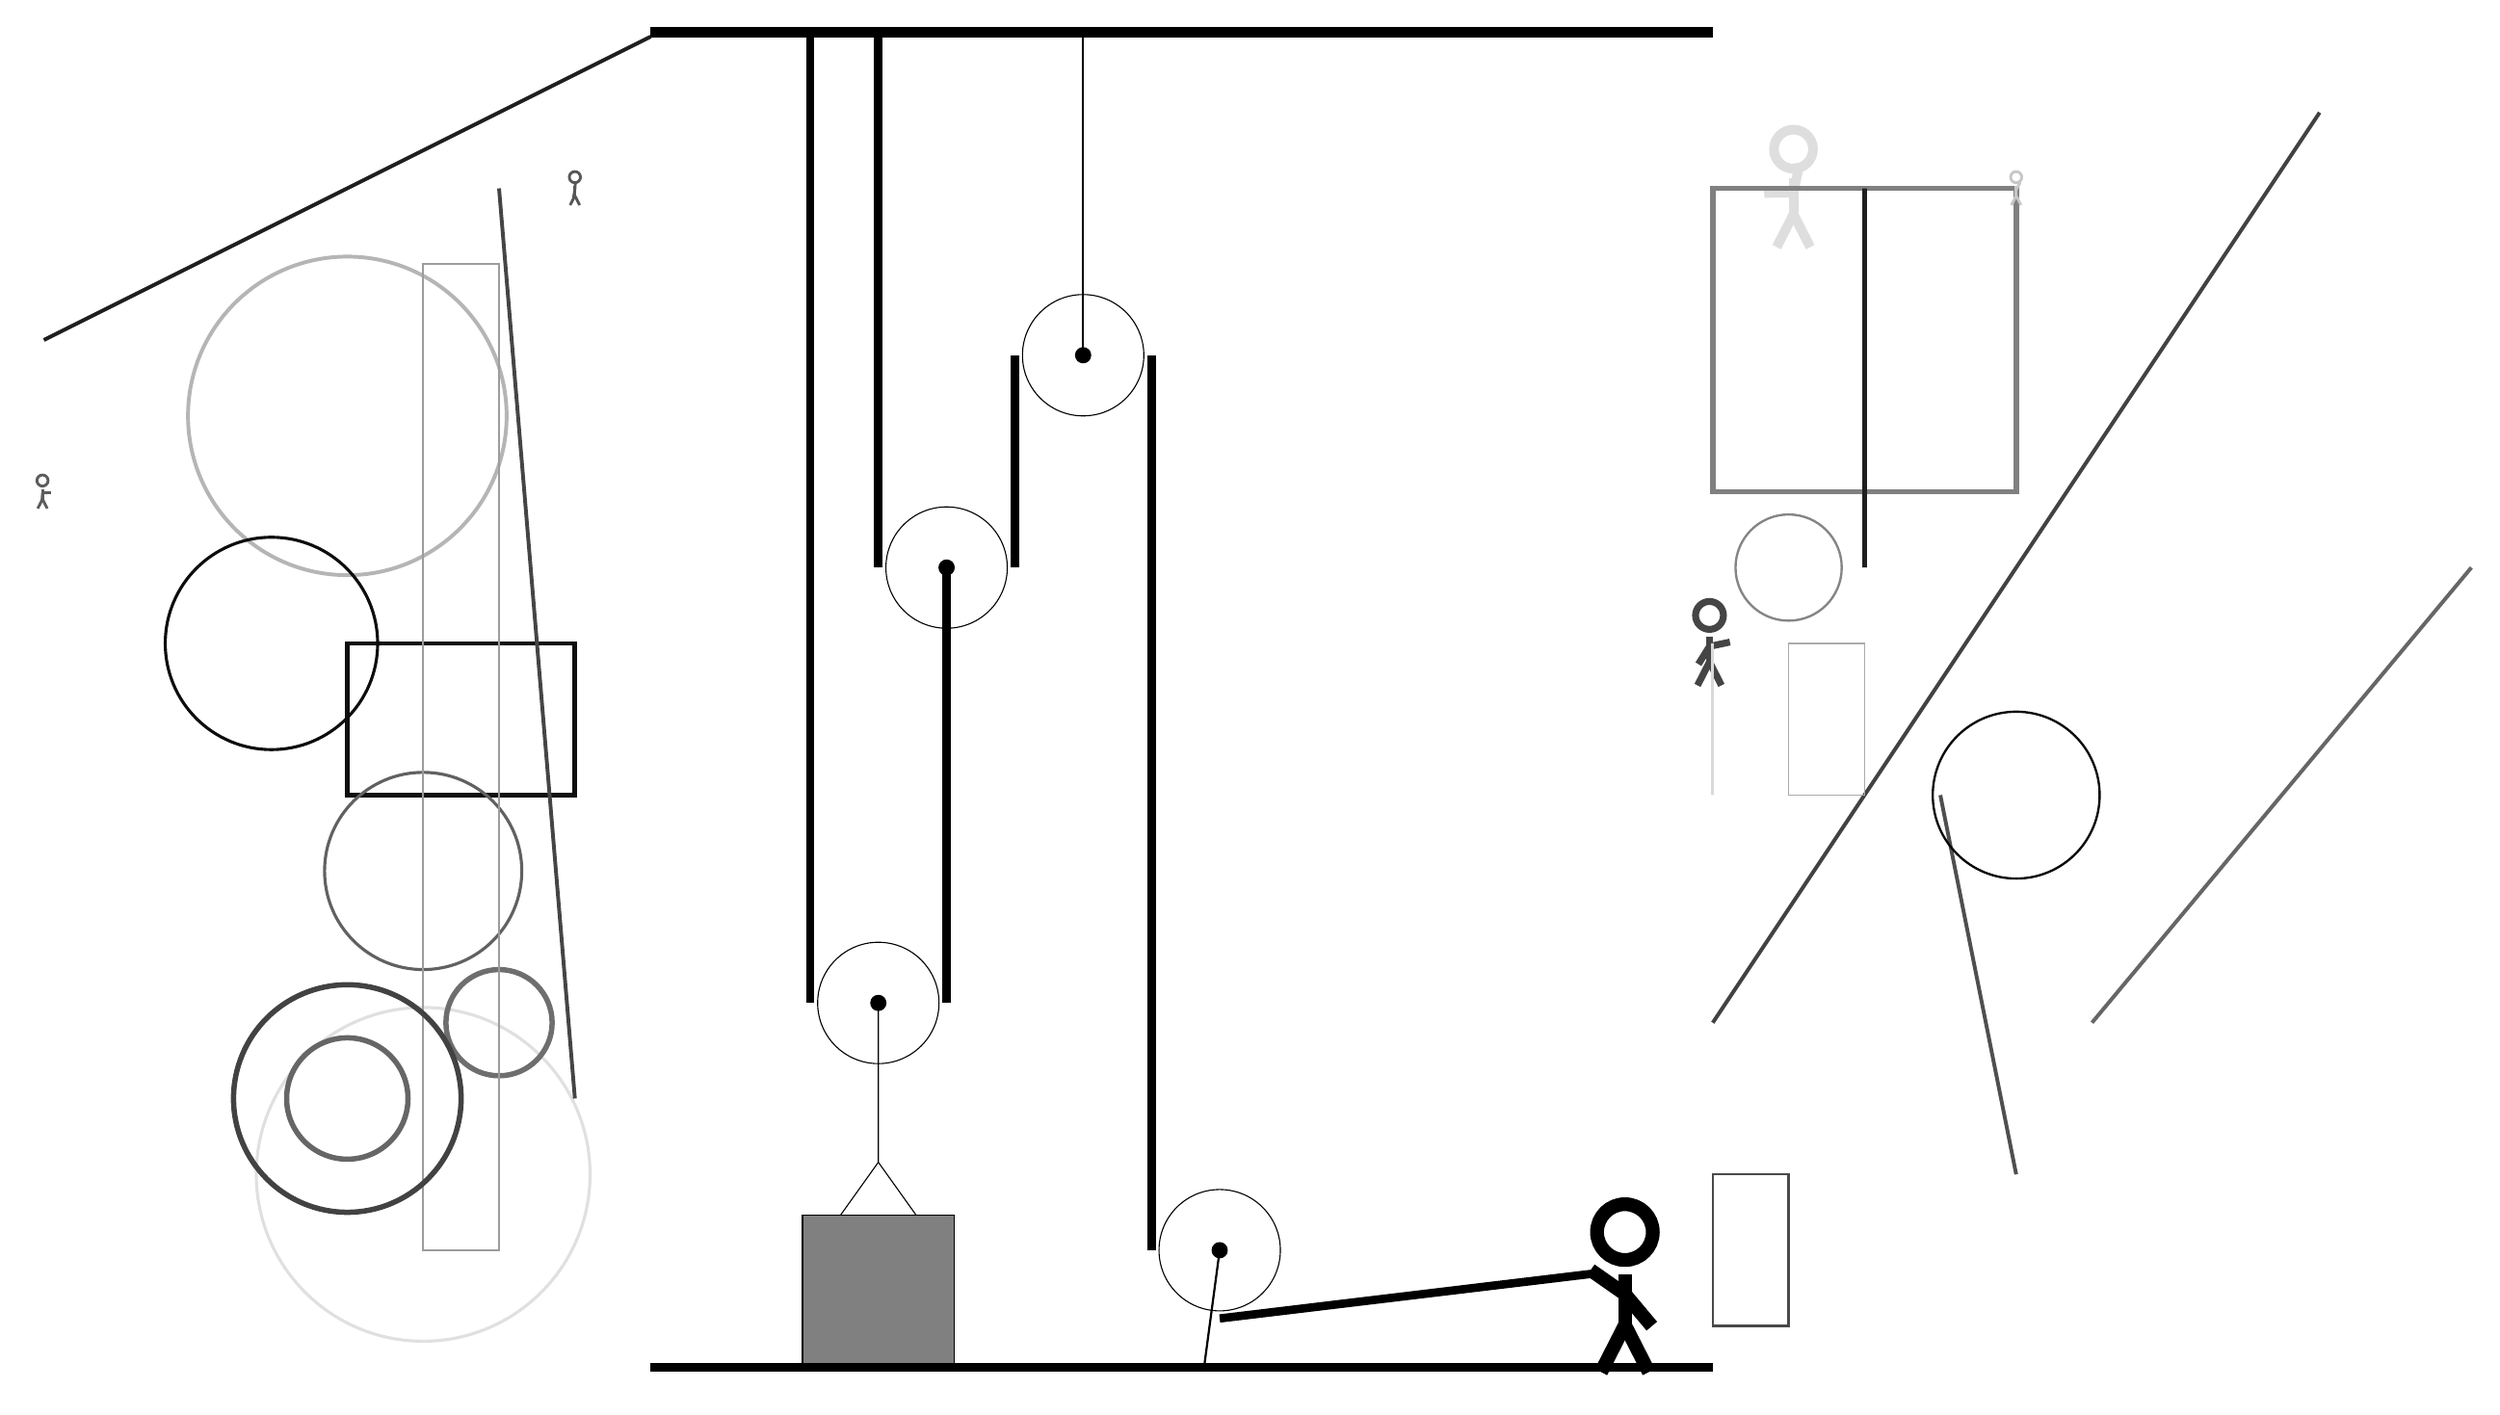
\begin{tikzpicture}
			%%%%% START %%%%%
			
			\draw[fill=black] (-2, 14) rectangle (12, 14.125);
			
			\draw (1, 1.26) circle (0.8);
			\draw[fill=black] (1, 1.26) circle (0.1);
			
			\draw (1.9, 7.0) circle (0.8);
			\draw[fill=black] (1.9, 7.0) circle (0.1);
			
			\draw (3.7, 9.8) circle (0.8);
			\draw[fill=black] (3.7, 9.8) circle (0.1);
			\draw[thick] (3.7, 9.8) -- (3.7, 14);
			
			\draw (5.5, -2) circle (0.8);
			\draw[fill=black] (5.5, -2) circle (0.1);
			\draw[thick] (5.5, -2) -- (5.3, -3.5);
			
			\draw (1, 1.26) -- (1, -0.84) -- (0.5, -1.54) -- (1.5, -1.54) -- (1, -0.84);
			\draw[fill=black!50] (0, -1.54) rectangle (2, -3.54);
			\draw[line width=1.1mm] (0.1, 14) -- (0.1, 1.26);
			\centerarc[line width=1.1mm](1, 1.26)(180:360:0.9);
			\draw[line width=1.1mm](1.9, 1.26) -- (1.9, 7.0);
			\draw[line width=1.1mm] (1.0, 14) -- (1.0, 7.0);
			\centerarc[line width=1.1mm](1.9, 7.0)(180:360:0.9);
			\draw[line width=1.1mm](2.8, 7.0) -- (2.8, 9.8);
			\centerarc[line width=1.1mm](3.7, 9.8)(0:180:0.9);
			\draw[line width=1.1mm] (4.6, 9.8) -- (4.6, -2);
			\centerarc[line width=1.1mm](5.5, -2)(0:90:-0.9);
			\draw[line width=1.1mm](5.5, -2.9) -- (10.5, -2.3);
			
			\draw [line width=0.3mm, color=black!48](13, 7) circle (0.7);
			
			\draw [line width=0.5mm, color=black!29](-6, 9) circle (2.1);
			\node[line width=0.5mm, color=black!13] at (13, 12) {\Strichmaxerl[7][1][78]};
			\draw[line width=0.6mm, color=black!94] (-3, 6) rectangle (-6, 4);
			\draw [line width=0.4mm, color=black!12](-5, -1) circle (2.2);
			\draw [line width=0.7mm, color=black!60](-6, 0) circle (0.8);
			\draw[line width=0.7mm, color=black!50] (12, 8) rectangle (16, 12);
			\draw [line width=0.4mm, color=black!95](-7, 6) circle (1.4);
			\draw[line width=0.5mm, color=black!74](12, 1) -- (20, 13);
			
			\draw [line width=0.7mm, color=black!57](-4, 1) circle (0.7);
			\draw[line width=0.5mm, color=black!60](17, 1) -- (22, 7);
			
			\node[line width=0.7mm, color=black!22] at (16, 12) {\Strichmaxerl[2][87][60]};
			\node[line width=0.4mm, color=black!73] at (12, 6) {\Strichmaxerl[5][58][12]};
			\draw[line width=0.4mm, color=black!15] (12, 4) rectangle (12, 6);
			\draw[line width=0.5mm, color=black!73](-3, 0) -- (-4, 12);
			\draw[line width=0.3mm, color=black!71] (12, -3) rectangle (13, -1);
			
			\draw [line width=0.4mm, color=black!62](-5, 3) circle (1.3);
			\draw[line width=0.2mm, color=black!39] (-4, -2) rectangle (-5, 11);
			\node[line width=0.4mm, color=black!64] at (-10, 8) {\Strichmaxerl[2][86][2]};
			
			\draw[line width=0.6mm, color=black!88] (14, 7) rectangle (14, 12);
			\draw[line width=0.5mm, color=black!88](-2, 14) -- (-10, 10);
			\draw [line width=0.7mm, color=black!74](-6, 0) circle (1.5);
			\draw[line width=0.2mm, color=black!33] (14, 6) rectangle (13, 4);
			\node[line width=0.7mm, color=black!66] at (-3, 12) {\Strichmaxerl[2][80][86]};
			\draw[line width=0.5mm, color=black!69](16, -1) -- (15, 4);
			
			\draw [line width=0.3mm, color=black!96](16, 4) circle (1.1);
			
			\node at (10.8, -2.5) {\Strichmaxerl[10][-35][-50]};
			
			\draw[fill=black] (-2, -3.5) rectangle (12, -3.6);
			
			%%%%% END %%%%%
		\end{tikzpicture}
	\end{figure}	
\end{document}